\chapter{Conception} \label{chap:conception}

\section*{}

In this chapter is are presented the process, rules and questionnaires that were conceived to enable semi-automatic SCAMPI evaluations. It is also presented an assessment of the level of support provided by SCRAIM regarding CMMI practices.

\section{Assessment Process} \label{sec:Approach}

The Electronic assessment process is represented in Figure \ref{fig:assessmentprocess}.
The process starts with a selection of the projects and process areas to evaluate. Then for each evaluation, we have two ongoing tasks; the survey based electronic assessment and the rule based assessment.

The survey based electronic assessment is a manual process (conducted with tool support) where the user needs to answer the questions that are provided. The rule based electronic assessment is fully automatic using the rules described later in this section.

Both assessments receive project data to generate the results that can be seen afterwards. In this workflow is present too the manual adjustment, a part that can be useful if in some case a certain part is not evaluated correctly or the assessment result is by consented opinion of the team accepted or rejected. And for last is shown the final results. 

The details of rule based and survey based assessment are provided in section \ref{sec:mapping} and \ref{sec:question}.

In order to get a full overview of SCRAIM, an assessment of the tool was performed. That assessment provides the current state of the tool and possible gaps to overcome.

\newpage
	\begin{figure}[H]
		\begin{center}
			\leavevmode
			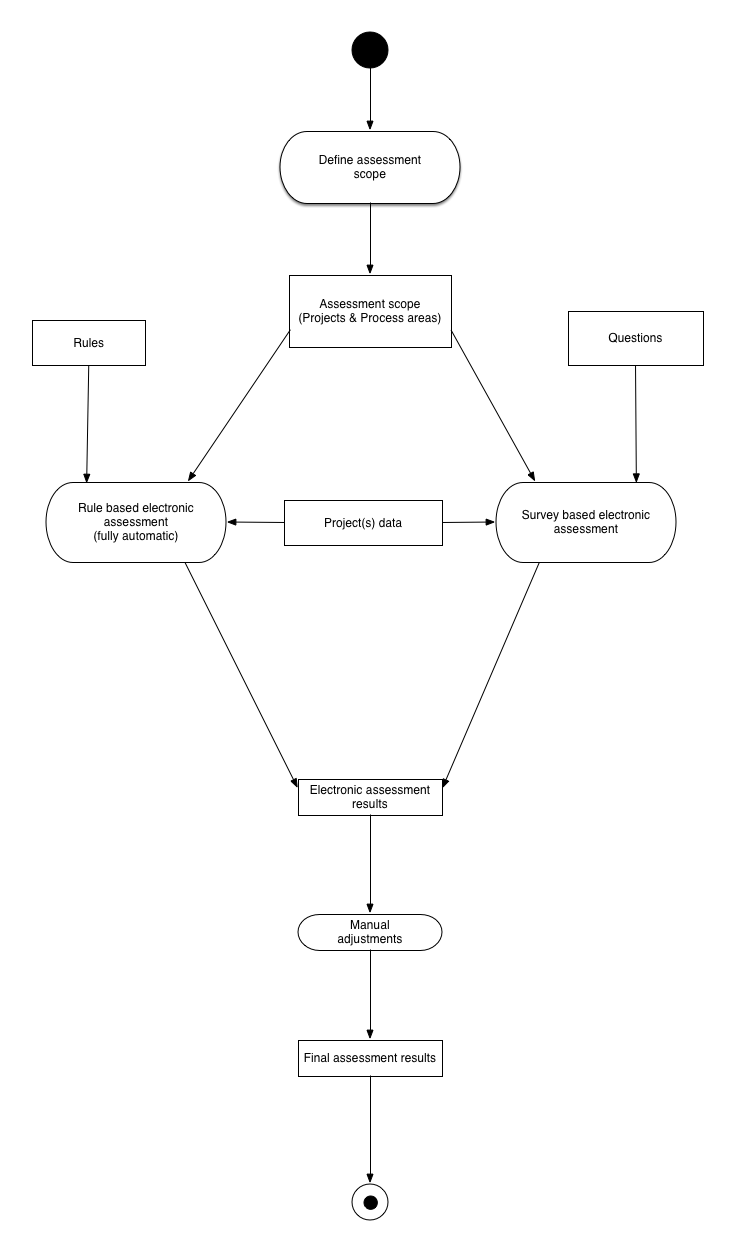
\includegraphics[width=0.9\textwidth]{assessprocess}
			\caption{UML activity diagram depicting the Assessment Process Workflow}
			\label{fig:assessmentprocess}
		\end{center}
	\end{figure}


\section{Pre-assessment of Scraim support} \label{sec:preassessment}

In a primary phase as mentioned before, an assessment of the tool was performed. The actual purpose of this assessment was to check if it was possible and currently viable to match Scraim and its functionalities with the third maturity level of CMMI for Development.

Maturity levels comprise a set of process areas, each with a set of goals and practices. So, if Scraim could be mapped to a more extensive number of practices and goals, a higher level of maturity could be covered.

The assessment was done with Appraisal Assistant, a tool currently used to assist and help appraisals in the field (see Section \ref{chap:chap3}). This tool allows us to visualize the results in a matrix, providing a full overview of the current state and the coverage of Scraim in relation to the maturity level 3 of CMMI for Development.


\begin{figure}[h]
	\begin{center}
		\leavevmode
		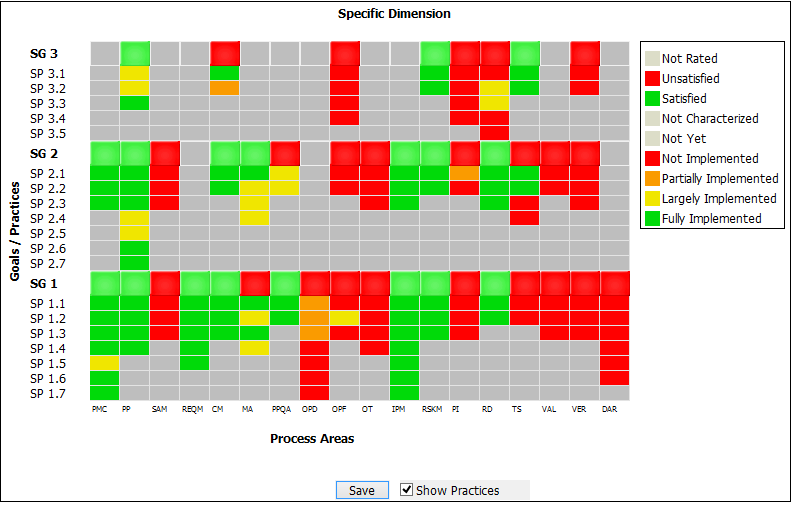
\includegraphics[width=0.8\textwidth]{Level_3}
		\caption{Scraim Assessment to CMMI for Development Level 3}
		\label{fig:level3}
	\end{center}
\end{figure}

In Figure \ref{fig:level3} we can see that, despite the fact that Scraim covers many practices, the maturity level three is still too far from being achieved successfully.

For example some areas like Verification (VER) and Decision Analysis and Resolution (DAR), are not currently supported by SCRAIM, so it will be impossible to automatically assess the fulfillment of their respective goals and practices by SCRAIM users.

In Figure \ref{fig:level2} we can see that the map for the second level of maturity is more accurate, more trustful and can be more covered automatically.
	
\begin{figure}[h]
	\begin{center}
		\leavevmode
		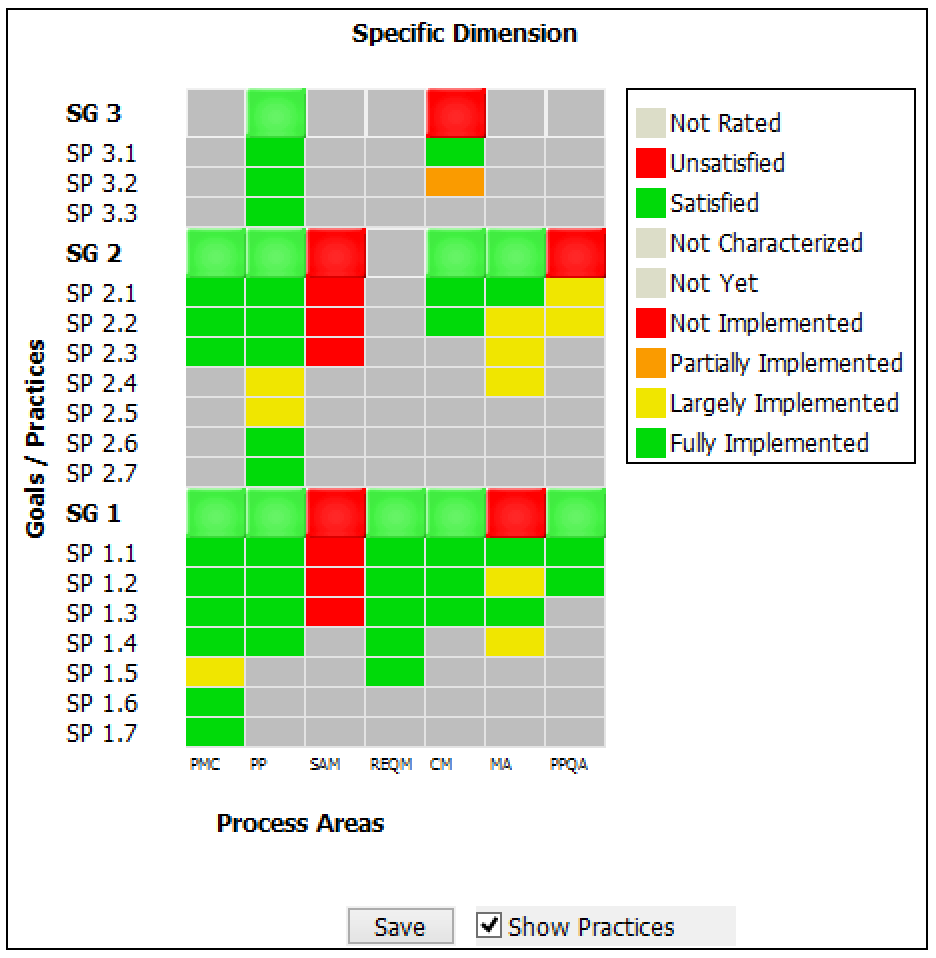
\includegraphics[width=0.6\textwidth]{Level_2}
		\caption{Scraim Assessment to CMMI for Development Level 2}
		\label{fig:level2}
	\end{center}
\end{figure}

The initial decision of making this set of tools to SCRAIM focusing in the level is supported by these two assessments to the tool.



\section{Electronic assessment rules} \label{sec:mapping}

In order to get rules it was needed to perform a mapping between CMMI concepts and SCRAIM data items. 

Taking as reference the previous assessments of the tool, this map was possible with the creation of a new scale to show the results of the assessment and be possible the map corresponding the information.

One appraisal consists in classifying each practice in one of four states: Fully Implemented, Largely Implemented, Partially implemented and Not implemented.

\begin{figure}[h]
	\begin{center}
		\leavevmode
		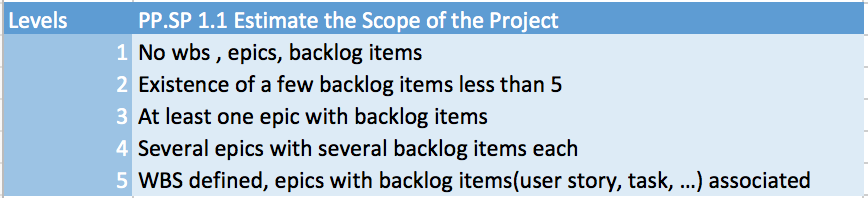
\includegraphics[width=0.6\textwidth]{mapping_5levels}
		\caption{Project Planning SP1.1 Map to 5 levels}
		\label{fig:mapping_5levels}
	\end{center}
\end{figure}

In the first attempt, was tried to match those levels with 5 levels, corresponding to different evaluation levels in Scraim. In the Figure \ref{fig:mapping_5levels} is possible to see the map between CMMI for Development and Scraim. In this example is analyzed the criteria from the practice 1.1 from the Project Planning area, which says, "Establish a top-level work breakdown structure (WBS) to estimate the scope of the project." and can be mapped into Scraim into this 5 levels. The first Level would be where there is none WBS item or backlog item, and the max level where all WBS are fully defined and epics with backlog items associated. 

\begin{figure}[h]
	\begin{center}
		\leavevmode
		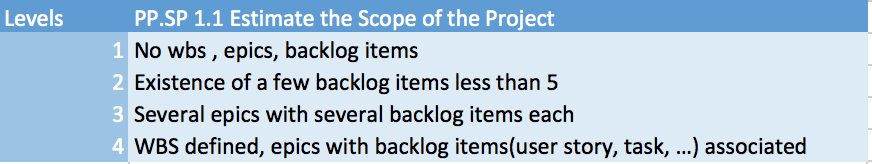
\includegraphics[width=0.6\textwidth]{mapping_4levels}
		\caption{Project Planning SP1.1 Map to 4 levels}
		\label{fig:mapping_4levels}
	\end{center}
\end{figure}

After some mapping this scale was confusing and far from real so the best way was to map and try match the four levels of SCAMPI with four levels of Scraim assessment.

This new scale is more accurate and closer to a real assessment as shown in Table \ref{tab:rules}. In Figure \ref{fig:mapping_4levels} is observable that the mid levels are more easily distinguished and more differentiable from the others.

\begin{table}[h]
	\centering
	\caption{Scale comparison}
	\begin{tabular}{|p{2cm}|p{4cm}|}
		\hline
		SCRAIM   & SCAMPI    \\
		\hline
		1 & Not Implemented\\
				\hline
				2 & Partially Implemented\\
				\hline
				3 & Largely Implemented\\
				\hline
				4 & Fully Implemented\\
				\hline
	\end{tabular}
	\label{tab:rules}
\end{table}

\section{Electronic assessment questions} \label{sec:question}

Regarding the mapping, it was discovered  that some practices can not be automatically evaluated so another way of providing some results needs to be found.

The founded way is make a survey based on pre-established questions. Those questions were derived from the "CMMI assessment checklist" (see Section \ref{cmmicheck}) and  the "ITMARK Appraisal tool" (see Section \ref{itmarktool}). One question example is presented in Figure \ref{fig:question_example}.

\begin{figure}[!htb]
	\begin{center}
		\leavevmode
		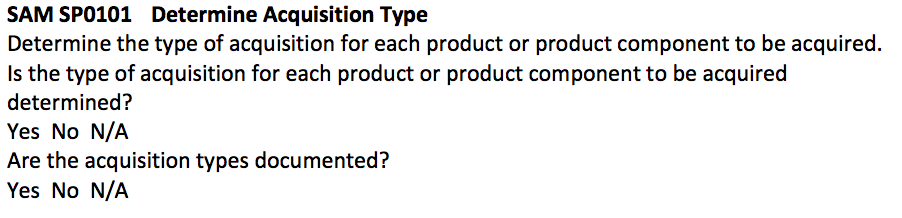
\includegraphics[width=0.6\textwidth]{question_example}
		\caption{Question example to cover Supplier Agreement Management Special Practice 1.1}
		\label{fig:question_example}
	\end{center}
\end{figure}

\section{Recommendations for extending the Scraim support}

Some of the gaps found in Section \ref{sec:mapping} can be solved with the integration of some plugins, frameworks and rules of usage, as follows:

\begin{itemize}
	\item Plugin for wiki templates \citep{wikitemplates}
	
	This plugin allows to choose a wiki template when a new page is added. It is possible to see a preview of the template before it is applied.
	This plugin will allow to resolve and insert some information directly in Scraim, without the use of other programs to generate those documents.
	
	\item Plugin for Document Management System Features \citep{DMSF}
	
	Allows to manage documents submitted on Scraim, document approval workflow to be configurable and maintain a version control of this documents.
	
	\item Certain names for submitted documents
	
	For example the Project plan must be submitted with a certain name to the Scraim files, to be automatically evaluated or it will not be considered.
	
\end{itemize}